\documentclass[a4paper, 11pt, oneside]{Thesis}  % Use the "Thesis" style, based on the ECS Thesis style by Steve Gunn
\graphicspath{Figures/}  % Location of the graphics files (set up for graphics to be in PDF format)
%\usepackage[T1]{fontenc}

\usepackage[square, numbers, comma, sort&compress]{natbib}  % Use the "Natbib" style for the references in the Bibliography
\usepackage{verbatim}  % Needed for the "comment" environment to make LaTeX comments
\usepackage{vector}  % Allows "\bvec{}" and "\buvec{}" for "blackboard" style bold vectors in maths
\usepackage{float}
\usepackage{multirow}
\usepackage{amsmath, amsthm, amssymb, pifont}
\usepackage{caption}
%\addbibresource{Bibliography.bib} % The filename of the bibliography
\usepackage[titletoc]{appendix}
\usepackage{color}
%\usepackage[style=authoryear]{biblatex}
%\usepackage[backend=bibtex,style=authoryear,natbib=true]{biblatex} % Use the bibtex backend with the authoryear citation style (which resembles APA)
%\addbibresource{example.bib} % The filename of the bibliography
%\usepackage[autostyle=true]{csquotes} % Required to generate language-dependent quotes in the bibliography

\DeclareMathOperator\arctanh{arctanh}
%\usepackage[labelfont=bf]{caption}
\captionsetup{
format = plain,
font = footnotesize,
figurename = FIGURE,
tablename = TABLE,
labelfont = {sc,bf}
}
%\usepackage[labelfont=bf,labelsep=space]{caption}
\hypersetup{urlcolor=blue, colorlinks=true}  % Colours hyperlinks in blue, but this can be distracting if there are many links.
\newcommand{\xmark}{\ding{55}}%
\newcommand{\chulo}{\ding{52}}%

%%----------------------------------------------------------------
\begin{document}
\frontmatter      % Begin Roman style (i, ii, iii, iv...) page numbering

\title  {Study of BCG-Substracted Images of Nearby Clusters}
%\authors  {\texorpdfstring
%            {\href{juancho9303@gmail.com}{Juan Manuel Espejo Salcedo}}
%            {Juan Manuel Espejo Salcedo}
%            }
            
\authors  
            {{Juan Manuel Espejo Salcedo}}
            
           
\addresses  {\groupname\\\deptname\\\univname}  % Do not change this here, instead these must be set in the "Thesis.cls" file, please look through it instead
\date       {\today}
\subject    {}
\keywords   {}

\maketitle
% ----------------------------------------------------------------

\setstretch{1.3}  % It is better to have smaller font and larger line spacing than the other way round

% Define the page headers using the FancyHdr package and set up for one-sided printing
\fancyhead{}  % Clears all page headers and footers
\rhead{\thepage}  % Sets the right side header to show the page number
\lhead{}  % Clears the left side page header

\pagestyle{fancy}  % Finally, use the "fancy" page style to implement the FancyHdr headers

% The "Funny Quote Page"
\pagestyle{empty}  % No headers or footers for the following pages

\null\vfill
% Now comes the "Funny Quote", written in italics
\textit{``Not only is the Universe stranger than we think, it is stranger than we can think..''}

\begin{flushright}
Werner Heisenberg
\end{flushright}

\vfill\vfill\vfill\vfill\vfill\vfill\null
\clearpage  % Funny Quote page ended, start a new page
%% ----------------------------------------------------------------

% The Abstract Page
\addtotoc{Abstract}  % Add the "Abstract" page entry to the Contents
\abstract{
\addtocontents{toc}{\vspace{1em}}  % Add a gap in the Contents, for aesthetics

We study the center of deep imaging data of low redshift massive galaxy clusters where the light from the BGC overwhelms the images from background galaxies and faint cluster members in the cluster core. The proper subtraction of the BCG light is expected to reveal background galaxies that are strongly lensed. We constrain the number of objects that we expect to find in these systems and corroborate these results when subtracting the BCGs and analysing these central regions. Identifying such systems allows for unique follow-up studies regarding the stellar populations in the BCGs and thus their formation history. Also the number density of faint cluster members may tell us something about the dynamical state of the cluster and how BGCs form. The aim of this project is to model the BCG light and search for strong lensing candidates and study the properties of faint cluster members in the core.

}

\clearpage  % Abstract ended, start a new page
%% ----------------------------------------------------------------

\setstretch{1.3}  % Reset the line-spacing to 1.3 for body text (if it has changed)

% The Acknowledgements page, for thanking everyone
\acknowledgements{
\addtocontents{toc}{\vspace{1em}}  % Add a gap in the Contents, for aesthetics

I would like to thank my supervisor Henk Hoekstra for his support and lessons during these months of research, for his kind supervision and his will to answer my questions. To my parents, who made my journey to the Netherlands possible and to my friends and teammates for a great time during the research \ldots

}
\clearpage  % End of the Acknowledgements
%% ----------------------------------------------------------------

\pagestyle{fancy}  %The page style headers have been "empty" all this time, now use the "fancy" headers as defined before to bring them back

%% ----------------------------------------------------------------
\lhead{\emph{Contents}}  % Set the left side page header to "Contents"
\tableofcontents  % Write out the Table of Contents

%% ----------------------------------------------------------------
%\lhead{\emph{List of Figures}}  % Set the left side page header to "List if Figures"
\listoffigures  % Write out the List of Figures

%% ----------------------------------------------------------------
%\lhead{\emph{List of Tables}}  % Set the left side page header to "List of Tables"
%\listoftables  % Write out the List of Tables

\setstretch{1.3}  % Return the line spacing back to 1.3

\pagestyle{empty}  % Page style needs to be empty for this page
\dedicatory{Dedicated to my parents, whose love and support are my biggest motivation\ldots}

\addtocontents{toc}{\vspace{2em}}  % Add a gap in the Contents, for aesthetics

%% ----------------------------------------------------------------
\mainmatter	  % Begin normal, numeric (1,2,3...) page numbering
\pagestyle{fancy}  % Return the page headers back to the "fancy" style

\lhead{\emph{Introduction}}
\chapter{Introduction}

Understanding the formation history of stars allows us to comprehend many physical properties of their host galaxies thus providing a useful framework on which to build a more elaborate theory of their subsequent evolution. We might have good ideas and some general agreement in the basics of formation of stars in galaxies, but our observational limitations don't allow us to say much about distant objects which we need to make a more elaborate and complete theory. In principle, we can't assume that all populations of stars have the same formation history in every galaxy and for every epoch of the Universe. The gas clouds that form stars might or might not create the same mixture of stars in every stellar system so it is important to see under what conditions we could assume a general trend and what implications in our observations this may have.

For galaxies that are far away, it is impossible to make star counts with our current technology, for this reason, their mass-to-light-ratio $\Upsilon$ (which depends on their stellar populations) provides a simple constraint on their number of stars per unit mass given by the initial mass function (IMF), which is a very fundamental and important quantity in the study of stellar systems because it constraints the physics of star formation but also because it allows us to infer stellar masses through observed luminosities as discussed by \textcolor{blue}{Smith \& Lucey} (\citeyear{Reference7}). Everything we know from galaxy evolution is implicitly assuming a certain form of the IMF with very little variations since it is the method we use to connect evolutionary sequences, this of course, given the fact that if every galaxy had its own IMF then it would be too difficult to study their evolution because of the lack of any knowledge about their history. 

A satisfactory determination of the IMF in galaxies is a difficult task, since it depends on very reliable and well-understood data and calibrations. The determination is usually made by observing star counts, getting the present-day luminosity function (assuming proper mass-luminosity relation and theoretical models that take into account the metallicity), getting the present-day mass function (for some evolutionary tracks and metallicities) and assuming some star formation history to get the IMF. All these assumptions, and the fact that extrapolating these results to systems in which we can't get star counts make the determination very complicated. Moreover, another difficulty of the determination of IMF is that the classical assumption of a single IMF covering the whole mass range is being questioned in favour of a two-component IMF to account for possible different formation modes.

Despite these difficulties, we have some observational information about IMFs in galaxies, in the case of spiral galaxies for example, the most commonly used IMFs are Chabrier (\textcolor{blue}{Chabrier} \citeyear{Reference31}) and Kroupa (\textcolor{blue}{Kroupa} \citeyear{Reference30}) which are decently constrained given the facilities of our observations in our own galaxy; also, bulges appear to have heavier IMFs than disks as mentioned by \textcolor{blue}{Brewer et. al.} (\citeyear{Reference16}). 

Although these primary assumptions given by our limited observational evidence might not be too far from reality, we must note that when we study more complex and dense systems like the brightest cluster galaxies (BCG) in galaxy clusters or giant elliptical galaxies in general, constraining the IMF via $\textrm{M}_{\star}/\textrm{L}$ might be way more complex and poses a greater challenge since masses are more difficult to establish for dynamically-hot systems like them. Measuring $\Upsilon$ in these systems is not a truly accurate constraint on the IMF since we may have different stellar formation histories than the ones associated with galaxies that are being formed now. These objects have a very old origin (although their build up and morphological formation is recent) because their stellar populations are old and they correspond to the highest density peak, so it is difficult to relate their stellar populations accurately.

The $\text{M}_{\star}/L$ depends on galaxy type, but due to the lack of multi-wavelength photometry, it is often assumed that all cluster galaxies are composed of the same stellar population. If one assumes an old stellar population (and therefore a high $\text{M}_{\star}/L$), the mass of the late-type galaxies (and thus the cluster as a whole) is over-estimated (\textcolor{blue}{Van der Burg et. al.} \citeyear{Reference2}).

Mass-to-light ratios of early-type galaxies are of particular interest to understand the tilt of the fundamental plane. Virial relations imply that the effective surface brightness $I_{\text{eff}}$, the effective radius $r_{\text{eff}}$ and the central velocity dispersion $\sigma_{0}$ in hot stellar systems are not independent of each other. This is revealed by the fundamental plane of early type galaxies.

This general view shows that in the context of the evolution of galaxies, there are many things that come together at the very core of cosmology but also in the context of stellar astrophysics and they need to be consistent with each other. Addressing this problem is complex for many reasons, one of them is that these systems have a strong dependency on their non-baryonic matter content which affects the mass-to-light-ratio determination. This dark matter contribution accounts for most of the dynamical mass of galaxies and it's the dominant contribution in most of their spacial scales, specially in the outer regions. The problem would be much easier to study if we only had the stellar mass because the light measurements would be enough to constrain the stellar populations, their evolution and their mass distribution. 

Being able to calculate the percentage of dark matter allows us to define the IMF more precisely. So we want to see what fraction of the surface density is given by stars and what are the spatial scales in which DM becomes the dominant contribution to the enclosed mass. DM halos seem to have a diluted profile in comparison to the stellar content of galaxies (\textcolor{blue}{Navarro Frenk \& White} \citeyear{Reference17}) so there is a region near the center of these massive systems in which the stellar mass is the dominant contribution. This implies that accurate measurements of their luminosity could give precise determinations of their mass to light ratio thus giving us some knowledge of their IMFs.

For stars, measurements of the luminosity function can be used to derive the Initial Mass Function (IMF). For galaxies, this is more difficult because Mass to light ratio (M/L) of the stellar population depends upon the star formation history of the galaxy. Bulges have heavier IMFs than disks. Recent studies have investigated how the IMF varies with galaxy mass, specially in elliptical galaxies. One of the methods used for this study is a rather indirect method, where galaxy stellar masses are determined from stellar population synthesis models that actually do not resolve the IMF, the results suggest that lower mass early-type galaxies (with dispersions $\sigma \approx 200$ km/s) seem to be consistent with a Milky-Way type IMF (e.g. a Kroupa or Chabrier IMF). In high-dispersion elliptical galaxies, however, stellar mass-to-light ratios are about a factor of 2 times higher than expected from a Kroupa IMF. Some studies indicate that the IMF in massive galaxies seems to be more dwarf dominated than in the Milky-Way so that they can be described by a Salpeter IMF (\textcolor{blue}{Thomas} \citeyear{Reference28}). Figure [1.1] shows the dependence of the enclosed mass of a galaxy on different IMFs.

\begin{figure}[H]
\centering
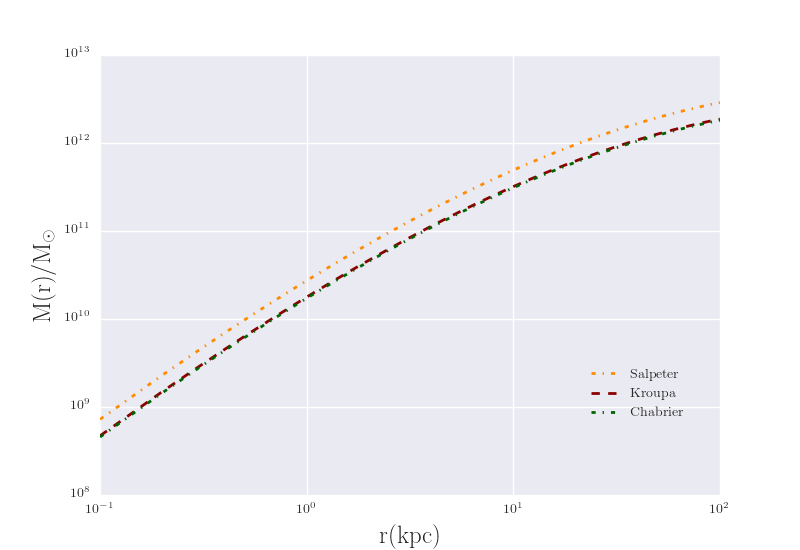
\includegraphics[width=12cm]{images/Enclosed_Mass_IMFs.png}
\caption[Enclosed mass for different IMFs in a galaxy]{Enclosed mass for different IMFs in a galaxy of $M_{200}\approx 10^{12} M_{\odot}$}
\end{figure}   

Various techniques have been developed to try to understand the stellar populations that form these massive systems. One of them is by using gravitational lensing  of  background galaxies (\textcolor{blue}{Treu et. al.} \citeyear{Reference1}). Modelling the lensing configuration on a BCG provides a useful method to determine stellar and dark matter mass contribution in elliptical galaxies, since it is difficult to constraint the IMF via $\textrm{M}_{\star}/\text{L}$ as mentioned before. Finding strong lensing in these systems can also give us information about the location of the mass center of the cluster through the lensing they produce. We usually assume that the centre of galaxy clusters lies in the BCGs (\textcolor{blue}{George et. al.} \citeyear{Reference18}) but the real position of the centre in galaxy clusters is still an unsolved problem (\textcolor{blue}{Harvey et. al} \citeyear{Reference13}). 

Strong lensing measures exactly the enclosed mass so we need to know how much of its contribution we need to subtract, the less we have to subtract, the better for the determination of the IMF. If the effect of the IMF is very subtle in the mass vs radius plot, then we would need to know the dark matter distribution very well, but if the effect of the IMF is not very subtle, the less we need to know about the dark matter distribution. A recent study of a BCG mentions the relevance of this spatial scale, at very small radii stars dominate the lensing mass, so that lensing provides a direct probe of the stellar mass-to-light ratio, with only small corrections needed for dark matter (\textcolor{blue}{Smith \& Lucey} \citeyear{Reference7}). 

In this project we work with galaxy clusters that might be in the right range to search for gravitational lensing in the inner regions. We use deep data from CFHT that allows us to search for interesting targets and probe the relevant spacial scales. We focus on the brightest cluster galaxy since it is a very massive system that could lens background objects and because photometry measurements can be made very accurately on them in comparison with their neighbouring galaxies. 

 % Introduction

\lhead{\emph{Introduction to Gravitational lensing}} 
\chapter{Introduction to Gravitational Lensing}

One of the most amazing results of Einstein's theory of general relativity, regarding the distortion of space time by massive objects is gravitational lensing. The basic principle behind gravitational lensing is that light is distorted when it travels close to the potential well (the distortion of space time) of massive objects (analogous to the effect of optical lenses). Under certain conditions the background objects can be seen in multiple images and ``arcs" surrounding the lensing object, this is known as strong gravitational lensing. 

For the general lens we first start by introducing the deflection angle which is the measure of the angular distance that has been deflected and which is linearly dependent on the mass $M$. This dependence ensures that the angles of deflection of an array of lenses can be superposed linearly. If we had N point masses sparsed one a plane, with positions $\xi$ and masses $M_{i}$, then the deflection angle would be:

equation 1

Fortunately, in most three dimensional distributions of matter (even in the case of lensing by massive objects like galaxy clusters) the physical size of the lens is generally much smaller than the distances between the observer, the lens and the source. This means that the deflection of light takes place in a very thin and short section of its path to the observer. Given this, we can use the \textit{thin screen approximation}: "The lens is approximated by a planar distribution of matter, the lens plane". Also the sources can be treated as if they lie on a plane which is called the source plane.

The \textit{thin screen approximation} allows us to state that the lensing matter distribution is fully described by its surface density

equation 2

where $\vec{\xi}$ is a two-dimensional vector on the lens plane and $\rho$ is the three dimensional density.

\begin{figure}[H]
\centering
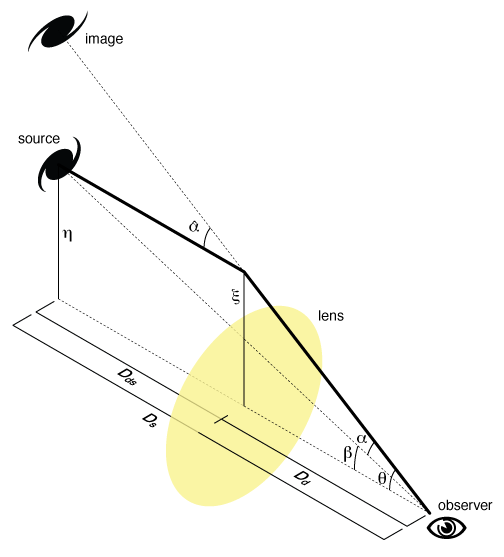
\includegraphics[width=12cm]{images/lensing.png}
\caption[Angles in gravitational lensing]{where $D_{ds}$ is the distance from the lense to the source $D_s$ is the distance from the observer to the source and $D_d$ is the distance from the observer to the source Wikipedia}
\end{figure}

Figure [] is a sketch of a typical gravitational system. The lensing mass is located at a angular diameter distance $D_d$ and it deflects the light rays coming from a source at an angular distance of $D_s$.

The optical axis is perpendicular to the lens and source planes and passes through the observer. We measure the angular positions on both planes with respect to this reference direction. The source is at the angular position $\vec{\beta}$ and lies on the source plane at a distance $\vec{\eta}=\vec{\beta}D_s$ from the optical axis. The deflection angle $\hat{\vec{\alpha}}$ of the light ray comes from the source and has impact parameter $\vec{\xi}=\vec{\theta}D_d$ on the lens plane. Due to this deflection, the observer receives the light coming from the source as if it was emitted at the angular position $\vec{\theta}$.

If $\vec{\theta}$, $\vec{\beta}$ and $\hat{\vec{\alpha}}$ are small, the true position of the source and its observed position on the sky are related by a very simple relation, obtained by a geometrical construction. This relation is called the lens equation and is written as

\begin{equation}
\vec{\theta}D_s = \vec{\beta}D_s+ \hat{\vec{\alpha}}D_{ds}     \\\\\\\\\\\
\end{equation}

where as seen in the figure, $D_{ds}$ is the distance between the lens and the source.

Defining the reduced deflection angle

\begin{equation}
\vec{\alpha}(\vec{\theta})\equiv \frac{D_{ds}}{D_s}\hat{\vec{\alpha}}(\vec{\theta})
\end{equation}

From equation ..... we get

\begin{equation}
\vec{\beta}=\vec{\theta}-\vec{\alpha}(\vec{\theta})
\end{equation}

The most interesting physics of the simple lens equation arises because $\vec{\alpha}$ depends on $\vec{\theta}$

Now, we can characterize an extender distribution of matter by it effective lensing potential, which is obtained by projecting the three-dimensional Newtonian potential on the lens plane and scaling it accordingly

\begin{equation}
\hat{\Psi}(\vec{\theta})=\frac{D_{ds}}{D_{d}D_{s}}\frac{2}{c^{2}}\int\Phi(D_{d}\vec{\theta},z)dz
\end{equation}

This lensing potential satisfies two important properties:

1) the gradient of $\Psi$ gives the scaled deflection angle:

\begin{equation}
\vec{\nabla}_{x}\Psi(\vec{x})=\vec{\alpha}(\vec{x})
\end{equation}

2) the Laplacian of $\varPsi$ gives twice the convergence

\begin{equation}
\Delta_{x}\Psi(\vec{x})=2\kappa(\vec{x})
\end{equation}

where the convergence is defined as a dimensionless surface density

\begin{equation}
\kappa(\vec{x})\equiv \frac{\Sigma(\vec{x})}{\Sigma_{cr}}\qquad \text{with} \qquad \Sigma_{cr}=\frac{c^{2}}{4\pi G}\frac{D_s}{D_d D_{ds}}
\end{equation}

$\Sigma_{cr}$ is called the critical surface density and it characterises the lens system and which is a function of the angular diameter distances of lens and source. 

Now let's talk about magnification and distortion.

One of the main features of gravitational lensing is that it distorts the shapes of the sources, this is particularly evident when the source has no negligible apparent size. In some cases the background galaxies can appear as very long arcs in galaxy clusters as mentioned at the beginning of this chapter. 

desde aca hay que modificar!!!!!!!!!!


The distortion takes place because light bundles are deflected differentially. Ideally the shape of the images can be determined by solving the lens equation for all the points within the extended source. In particular, if the source is much smaller than the angular size on which the physical properties of the lens change, the relation between the source and image positions can locally be linearised. In other words, the distortion of images can be described by the Jacobian matrix
\begin{equation}
A\equiv\frac{\partial\vec{y}}{\partial\vec{x}}=\left(\delta_{ij}-\frac{\partial\alpha_{i}(\vec{x})}{\partial x_{j}}\right)=\left(\delta_{ij}-\frac{\partial^{2}\Psi(\vec{x})}{\partial x_{i}\partial x_{j}}\right)
\end{equation}

where $x_i$ indicates the $i$-component of $\vec{x}$ on the lens plane. it shows that the elements of the Jacobian matrix can be written as combinations of the second derivatives of the lensing potential. For brevity, we will use the shorthand notation

\begin{equation}
\frac{\partial^{2}\Psi(\vec{x})}{\partial x_{i}\partial x_{j}}\equiv\Psi_{ij}
\end{equation}

We can now split off an isotropic part from the Jacobian:

\begin{equation}
\left(A-\frac{1}{2}trA\cdot I\right)_{ij}=\left(\begin{array}{cc}
-\frac{1}{2}\left(\Psi_{11}-\Psi_{22}\right) & -\Psi_{12}\\
-\Psi_{12} & \frac{1}{2}\left(\Psi_{11}-\Psi_{22}\right)
\end{array}\right)
\end{equation}

which is an antisymmetric, trace-free matrix called the shear matrix. It quantifies the projection of the gravitational tidal field (the gradient of the gravitational force), which describes distortions of background sources.  This allows us to define the pseudo-vector $\vec{\gamma}=(\gamma_1 , \gamma_2)$ on the lens plane, whose components are

\begin{equation}
\gamma_1(\vec{x})=\frac{1}{2}(\Psi_{11}-\Psi_{22})\qquad and \qquad \gamma_2(\vec{x})=\Psi_{12} = \Psi_{21}
\end{equation}

This is called the shear. The eigenvalues of the shear matrix are 

\begin{equation}
\pm \sqrt{\gamma_1^2 + \gamma_2^2} = \pm \gamma
\end{equation}

Thus, there exists a coordinate rotation by an angle $\phi$ such that 

\begin{equation}
\left(\begin{array}{cc}
\gamma_{1} & \gamma_{2}\\
\gamma_{2} & -\gamma_{1}
\end{array}\right)=\gamma\left(\begin{array}{cc}
\cos2\phi & \sin2\phi\\
\sin2\phi & -\cos2\phi
\end{array}\right)
\end{equation}

And for the trace we have

\begin{equation}
\frac{1}{2}trA=(1-\kappa)\delta_{ij}
\end{equation}

This the Jacobian becomes 

\begin{equation}
A= \left(\begin{array}{cc}
1-\kappa-\gamma_{1} & -\gamma_{2}\\
-\gamma_{2} & 1-\kappa+\gamma_{1}
\end{array}\right)
\end{equation}

Where $\kappa$ is the convergence that determines the magnification and $\gamma_{1}$ and $\gamma_{2}$ are the shear components that determine the distortion of the background objects. This is an antisymmetric, trace-free matrix that quantifies the projection of the gravitational tidal field (the gradient of the gravitational force), which describes distortions of background sources.

Finally, we can introduce another useful quantity in the characterization of gravitational lensing systems. The \textit{magnification} is quantified by the inverse of the determinant of the Jacobian matrix. For this reason, the matrix $M=A^{-1}$ is called the \textit{magnification tensor}, and we define

\begin{equation}
\mu \equiv \text{det} M = \frac{1}{\text{det}A}=\frac{1}{(1-\kappa)^2-\gamma^2}
\end{equation}

The eigenvalues of the magnification tensor measure the amplification in the tangential and in the radial direction and are given by

\begin{equation}
\mu_t = \frac{1}{\lambda_t}=\frac{1}{1-\kappa - \gamma} \qquad and \qquad  \mu_r = \frac{1}{\lambda_r}=\frac{1}{1-\kappa + \gamma}
\end{equation}

The magnification is ideally infinite where $\lambda_t=0$ and where $\lambda_r=0$. These two conditions define two curves in the lens plane, called the tangential and the radial critical line, respectively. An image forming along the tangential critical line is strongly distorted tangentially to this line. On the other hand, an image forming close to the radial critical line is stretched in the direction perpendicular to the line itself. 

There are three classes of gravitational lensing:

1. \textbf{Strong lensing:} where there are easily visible distortions such as the formation of Einstein rings, arcs, and multiple images.

2.\textbf{ Weak lensing:} where the distortions of background sources are much smaller and can only be detected by analysing large numbers of sources in a statistical way to find coherent distortions of only a few percent

3. \textbf{Very weak lensing:} 

\begin{figure}[H]
\centering
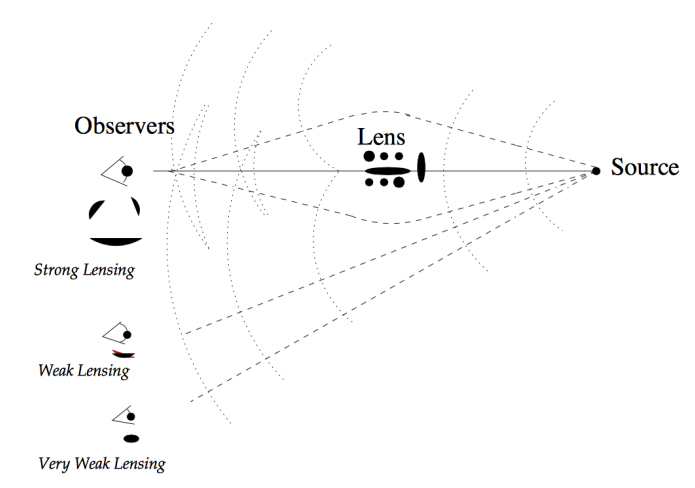
\includegraphics[width=12cm]{images/types_of_lensing.png}
\caption[Types of lensing]{Types of lensing. Courbin, F. et al \citeyear{Reference24}}
\end{figure}

Figure [] is a representation of a lensing system in which a background galaxy is lensed by a cluster of galaxies and produces multiple images as observed from Earth. 

\begin{figure}[H]
\centering
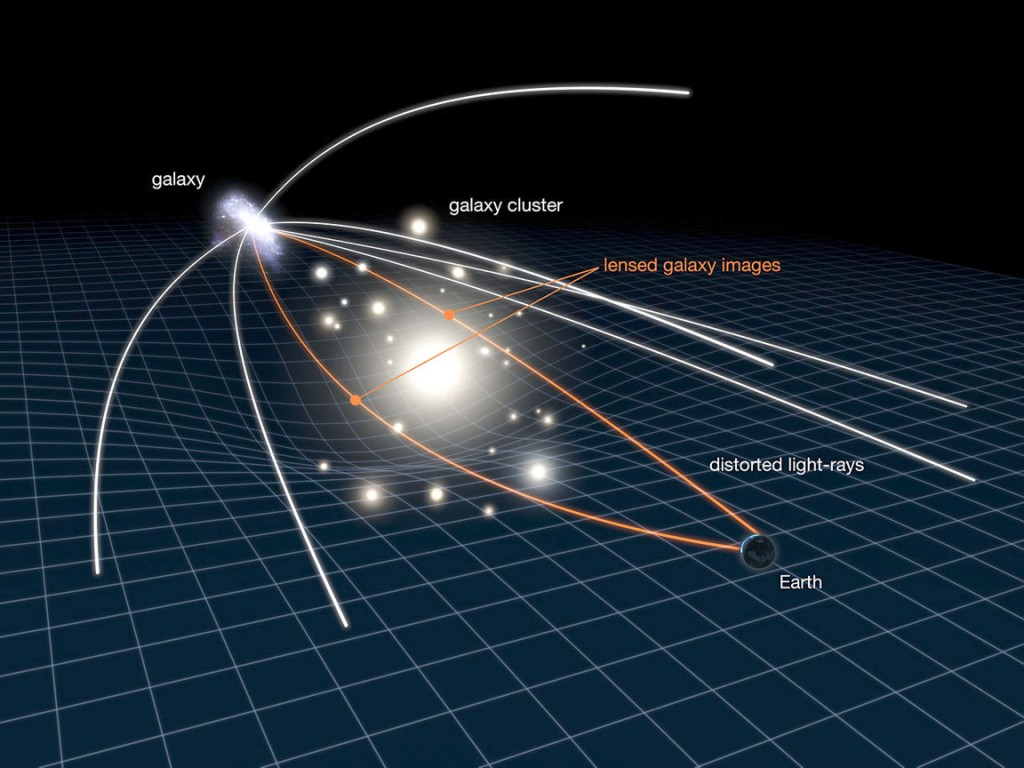
\includegraphics[width=12cm]{images/strong_lensing.jpg}
\caption[Strong Lensing representation]{Nasa?}
\end{figure}

Figure [] is a composite image of a galaxy cluster taken by the HST in which many lensed objects can be seen as distorted shapes and multiple images. 

\begin{figure}[H]
\centering
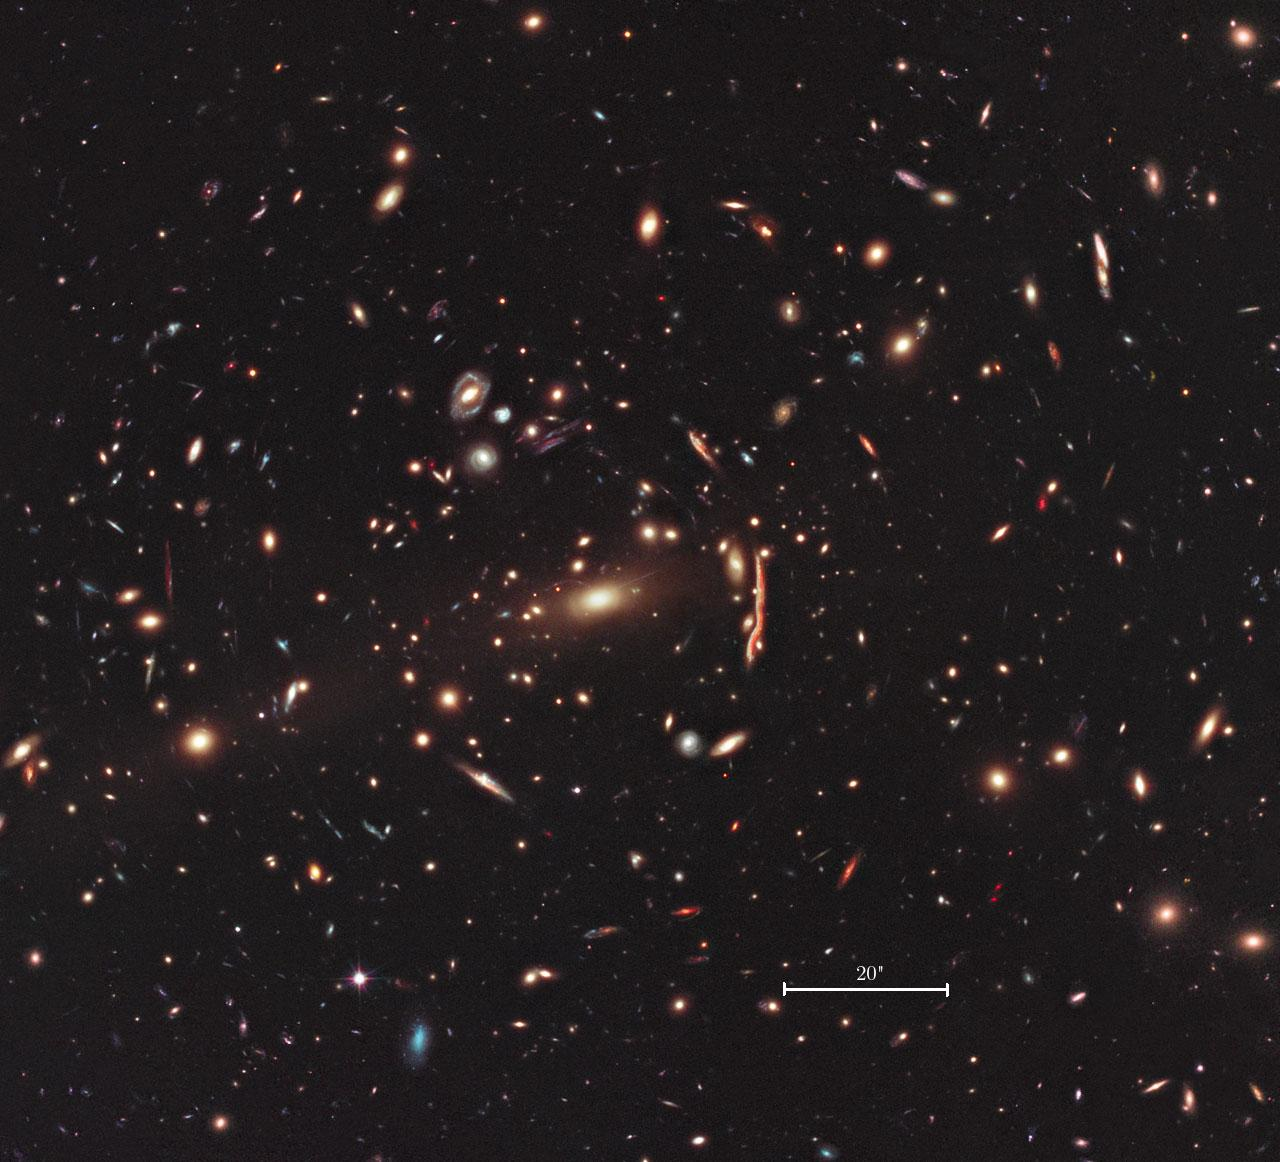
\includegraphics[width=12cm]{images/GC.jpg}
\caption[Galaxy Cluster MACS 1206]{Galaxy Cluster MACS 1206, credits to NASA Hubble Space Telescope}
\end{figure}

Quoted (need to change this): The image of galaxy cluster MACS J1206.2-0847 (or MACS 1206) is part of a broad survey with NASA Hubble Space Telescope. The distorted shapes in the cluster are distant galaxies from which the light is bent by the gravitational pull of an invisible material called dark matter within the cluster of galaxies. This cluster is an early target in a survey that will allow astronomers to construct the most detailed dark matter maps of more galaxy clusters than ever before.These maps are being used to test previous, but surprising, results that suggest that dark matter is more densely packed inside clusters than some models predict. This might mean that galaxy cluster assembly began earlier than commonly thought.

Scientists are planning to observe a total of 25 galaxy clusters under a project called CLASH (Cluster Lensing and Supernova survey with Hubble). One of the first objects observed for the new census is the galaxy cluster MACS J1206.2-0847. This conglomeration of galaxies is one of the most massive structures in the universe, and its gigantic gravitational pull causes stunning gravitational lensing. MACS 1206 lies 4 billion light-years from Earth. In addition to curving of light, gravitational lensing often produces double images of the same galaxy. In the new observation of cluster MACS J1206.2-0847, astronomers counted 47 multiple images of 12 newly identified galaxies.The era when the first clusters formed is not precisely known, but is estimated to be at least 9 billion years ago and possibly as far back as 12 billion years ago. If most of the clusters in the CLASH survey are found to have excessively high accumulations of dark matter in their central cores, then it may yield new clues to the early stages in the origin of structure in the universe.

Galaxies and clusters of galaxies that act as gravitational lenses can be approximated by single isothermal spheres. It is easy to relate an angular scaling parameter $\xi_{E}$, referred to as the Einstein radius, to the mass inside the corresponding light cone. The Einstein radius corresponds to the ring image of a point source aligned exactly on the axis of the lens.

Summary of isothermal sphere:

\begin{equation}
\rho(r)=\frac{\sigma^2}{2\pi Gr^2}
\end{equation}

\begin{equation}
\Sigma(\xi)=\frac{\sigma^2}{2G\xi}
\end{equation}

\begin{equation}
\xi_{E}=4\pi\left(\frac{\sigma}{c}\right)^{2}\frac{D_{ds}}{D_{s}}
\end{equation}

In reality, the density profile and lensing properties of galaxies is a bit more complicated than the assumption of a singular isothermal sphere, so we need to take into account more complex but elaborate profiles such as the NFW (Navarro, Frenk, White, \citeyear{Reference17}).

The NFW density profile is 

\begin{equation}
\rho(r)=\frac{\delta_{c}\rho_{c}}{(r/r_{s})(1+r/r_{s})^{2}}
\end{equation}

where the characteristic over density (dimensionless quantity) is given by:

\begin{equation}
\delta_{c}=\frac{200}{3}\frac{c^{3}}{\ln{(1+c)}-c/(1+c)}
\end{equation}

The mass of an NFW halo contained within a radius of $r_{200}$ is:

\begin{equation}
\text{M}_{200}=\text{M}(r_{200})=\frac{800\pi}{3}\rho_{c}r^{3}_{200}=\frac{800\pi}{3}\frac{\bar{\rho}(z)}{\Omega(z)}r^{3}_{200}
\end{equation}

The concentration parameter $c$ is strongly correlated with Hubble type, c=2.6 separating early from late-type galaxies. Those galaxies with concentration indices $c>2.6$ are early-type galaxies reflecting the fact that the light is more concentrated towards their centres, its formal definition in terms of the virial and characteristic radius is $c=r_{200}/r_{s}$.

Dutton \& Maccio \citeyear{Reference23} (in continuation of previous studies such as Mu\~noz Cuartas et. al. \citeyear{Reference12}), made simulations of halo masses from dwarf galaxies to galaxy clusters and find constraints on the concentration parameter for different redshifts, the relation between the concentration parameter with redshift and virial mass is shown in figure [].

\begin{figure}[H]
\centering
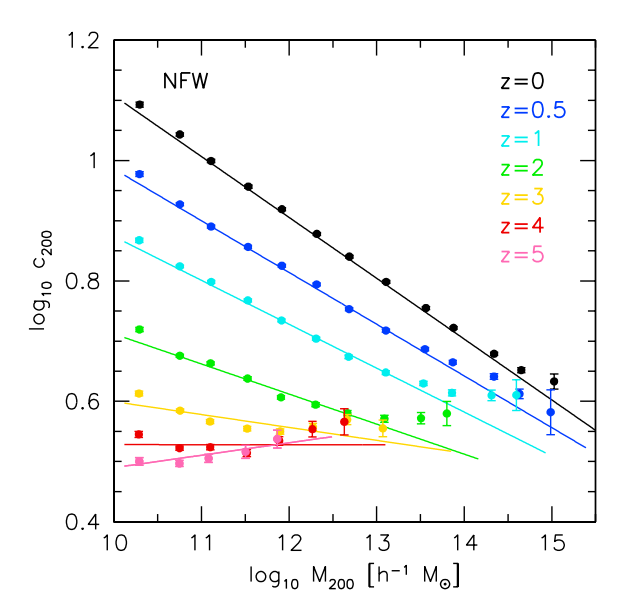
\includegraphics[width=10cm]{images/dutton.png}
\caption[Evolution of the concentration mass relation]{Evolution of the concentration mass relation, by Dutton \& Maccio, \citeyear{Reference23}}
\end{figure}

The surface mass density in the NFW profile is given by:

\begin{equation}
\Sigma_{\text{NFW}}(x) = \left\lbrace
\begin{array}{lll}
\frac{2r_{s}\delta_{c}\rho_{c}}{\left(x^{2}-1\right)}\left[1-\frac{2}{\sqrt{1-x^{2}}}\arctanh\sqrt{\frac{1-x}{1+x}}\right] & (x<1)\\\\
\frac{2r_{s}\delta_{c}\rho_{c}}{3} & (x=1)\\\\
\frac{2r_{s}\delta_{c}\rho_{c}}{\left(x^{2}-1\right)}\left[1-\frac{2}{\sqrt{x^{2}-1}}\arctan\sqrt{\frac{x-1}{1+x}}\right] & (x>1)
\end{array}
\right.
\end{equation} 

so from the critical density:

\begin{equation}
\rho_{c}=\frac{3H^2(z)}{8\pi G}
\end{equation}

$H(z)=H_{0}(1+\Omega z)^{3/2}$

But we are more interested in the enclosed mass which can be done by integrating the surface mass density:

\begin{equation}
\text{M}(R)=\int_{0}^{R}2\pi R\Sigma(R)dR
\end{equation}

The radial dependence on the shear is:

\begin{equation}
\gamma_{\text{NFW}}(x) = \left\lbrace
\begin{array}{lll}
\frac{r_{s}\delta_{c}\rho_{c}}{\Sigma_c}g_{<}(x) & (x<1)\\\\
\frac{r_{s}\delta_{c}\rho_{c}}{\Sigma_c}\left[\frac{10}{3}+4 \ln \left(\frac{1}{2}\right)\right] & (x=1)\\\\
\frac{r_{s}\delta_{c}\rho_{c}}{\Sigma_c}g_{>}(x) & (x>1)
\end{array}
\right.
\end{equation} 

where: 

\begin{equation}
g_{<}(x)=\frac{8 \arctanh \sqrt{\frac{1-x}{1+x}}}{x^{2}\sqrt{1-x^{2}}}+\frac{4}{x^{2}} \ln \left(\frac{x}{2}\right)-\frac{2}{\left(x^{2}-1\right)}+\frac{4 \arctanh \sqrt{\frac{1-x}{1+x}}}{\left(x^{2}-1\right)\left(1-x^{2}\right)^{1/2}}
\end{equation}

\begin{equation}
g_{<}(x)=\frac{8 \arctan \sqrt{\frac{x-1}{1+x}}}{x^{2}\sqrt{x^{2}-1}}+\frac{4}{x^{2}}\ln \left(\frac{x}{2}\right)-\frac{2}{\left(x^{2}-1\right)}+\frac{4 \arctan \sqrt{\frac{x-1}{1+x}}}{\left(x^{2}-1\right){}^{3/2}}
\end{equation} 

and with the critical surface mass density:

\begin{equation}
\Sigma_{c}\equiv\frac{c^{2}}{4\pi G}\frac{D_{s}}{D_{d}D_{ds}}
\end{equation}

these equations come from the paper Wright and Brainerd 1999.

The magnification tensor is:

\begin{equation}
\frac{\partial\beta}{\partial\theta}=\delta_{ij}-\frac{\partial^{2}\psi}{\partial\theta_{i}\partial\theta_{j}}=\left(\begin{array}{cc}
1-\kappa-\gamma_{1} & -\gamma_{2}\\
-\gamma_{2} & 1-\kappa+\gamma_{1}
\end{array}\right)
\end{equation}

The total magnification $\mu$ is given by the determinant of the magnification tensor:

\begin{equation}
\mu = \frac{1}{(1-\kappa)^{2}-\gamma^{2}_{1}-\gamma^{2}_{2}}
\end{equation}



 % Introduction to Gravitational lensing

\lhead{\emph{Determination of the relevant scales}}
%\usepackage{subfig}

\chapter{Observational Procedures}

\section{Sextractor}

\section{Galfit}

\section{Color images}


In er.   % Determination of the relevant scales
 
\lhead{\emph{Data and analysis}} 
\chapter{Data and analysis}

For this project we make use of good quality deep data of galaxy clusters observed with the MegaCam wide field imager on the CFHT (Canada-France-Hawii Telescope). The cluster sample consisted of 101 clusters within the range of redshifts from $0.05<z<0.55$. The full description of this survey can be found in \textcolor{blue}{Sand et al.} (\citeyear{Reference11})

58 clusters from the MENEACS (Multi-Epoch Nearby Cluster Survey). The MENEACS clusters represent all clusters in the BAX X-ray cluster database that are observable for the CFHT and this part of the data is in the $g$ and $r$ bands. We also make use of the INT data of the same cluster in the $i$ and $U$ bands. 

After filtering out some of the clusters because of a very complex and crowded central region or just not good quality we used 30 clusters for the final studies and paid special attention to 10, marked with * in Table [4.1].

The original images have dimensions of [20000:20000] pixels but since our relevant region is the center of the cluster where the BCG is located, we cut the images with dimension of [1000,1000] for the color analysis and [4000:4000] to characterize the colors and discriminate between cluster and non-cluster members. The pixel scale for CFHT is 0.185 arcsec/pix and 0.33 arcsec/pix for the INT data so the proper conversion must be done to match them accordingly.

\begin{table}[H]
\centering

\begin{tabular}{ccccc}
Cluster & $z$   & $\sigma(km/s)$ & $d(Mpc)$ & $\theta_{E}(")$ \\ \hline \hline
A1033   & 0.126 & 762            & 540 & 14.6155  \\
A1068*  & 0.138 & 740            & 591.4 & 13.5945  \\
A1132   & 0.136 & 727            & 582.9 & 13.1515   \\
A119*   & 0.044 & 875            & 188.6 & 21.0798   \\
A1413*  & 0.143 & 881            & 612.9 & 19.1569   \\
A1650   & 0.084 & 720            & 360 & 13.6758   \\
A1651   & 0.085 & 903            & 364.3 & 21.4876   \\
A1795   & 0.062 & 778            & 265.7 & 16.3514   \\
A2029*  & 0.077 & 1152           & 330 & 35.2776   \\
A2050   & 0.118 & 854            & 505.7 & 18.5258   \\
A2055   & 0.102 & 697            & 437.1 & 12.5642   \\
A2064   & 0.108 & 675            & 462.9 & 11.7048   \\
A2065*  & 0.073 & 1095           & 312.9 & 32.0110   \\
A2069   & 0.116 & 966            & 497.1 & 23.7574   \\
A2142*  & 0.091 & 1086           & 390 & 30.8756   \\
A2319*  & 0.056 & 1101           & 240 & 32.9563   \\
A2420   & 0.085 & ~800           & 364.3 & 16.8653   \\
A2440   & 0.091 & 766            & 390 & 15.3608   \\
A2597   & 0.085 & 682            & 364.3 & 12.2569   \\
A2627   & 0.126 & ~800           & 540 & 16.1096   \\
A2703   & 0.114 & ~800           & 488.6 & 16.3307   \\
A399    & 0.072 & ~800           & 308.6 & 17.1049   \\
A553    & 0.066 & ~800           & 282.9 & 17.2155   \\
A655*   & 0.127 & ~800           & 544.3 & 16.0911   \\
A754*   & 0.054 & ~800           & 231.4 & 17.4367   \\
A763    & 0.085 & ~800           & 364.3 & 16.8653   \\
A795    & 0.136 & ~800           & 582.9 & 15.9252   \\
A85*    & 0.055 & ~800           & 235.7 & 17.4182   \\
A961    & 0.124 & ~800           & 531.4 & 16.1464   \\
A990    & 0.144 & ~800           & 617.1 & 15.7778   
\end{tabular}
\caption[Abell Clusters and their redshift]{Abell clusters used in this work. Marked with * the chosen clusters with the most promising features. From left to right: Name of the cluster, redshift, velocity dispersions from \textcolor{blue}{Sifon et al.} (\citeyear{Reference6}), distance in Mpc and Einstein Ring using a single isothermal sphere as first approximation.}
\end{table}

The INT images were obtained using multiple exposures so it was necessary to make a mosaic of them using \texttt{SWARP} \textcolor{blue}{Bertin et al.} (\citeyear{Reference29}), so at the end we had the data of the clusters in the bands $g,r,U,i$ with the same spatial scale. The first step in the removal of the light from the BCG was constructing a mask file (segmentation file) to only extract the desired galaxy, this was done using \texttt{SEXTRACTOR} (\textcolor{blue}{Bertin \& Arnouts} \citeyear{Reference27}). 

The procedure is the following: \texttt{SEXTRACTOR} identifies the bright objects and extracts them while doing aperture photometry on them, the user can choose to obtain an examination image to see the extracted objects (that in our case would be the segmentation file). \texttt{SEXTRACTOR} labels each of the extracted regions with growing numbers where 1 is the brightest object (in most cases the BCG) so we can use python scripts to modify the segmentation file to mask only the galaxies but not the BCG which we want to fit properly. Figure [4.1] shows the original segmentation image and the one where the BCG light has been removed so that it won't be masked once we fit the light of the BCG (cluster Abell 754). 

\begin{figure}[H]
\centering
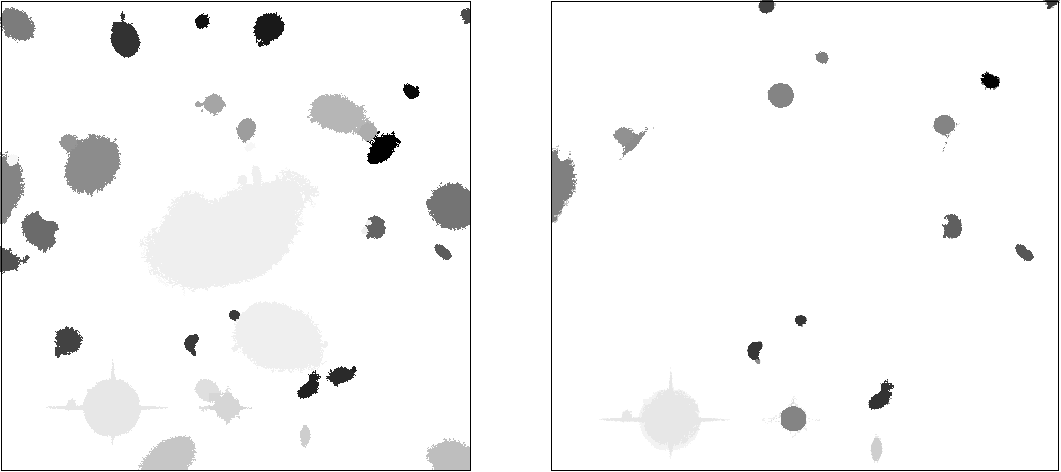
\includegraphics[width=15cm]{images/masks.png}
\caption[Segmentation images]{Segmentation images produced by \texttt{SEXTRACTOR} and used as mask files for the galfit extraction on the cluster Abell 754. Left panel is the original mask with all the bright objects. Right panel is the mask after the subtraction of the regions surrounding the cluster galaxies to be fitted with \texttt{GALFIT}. The colors are inverted for an easier visualization of the image. The fainter regions are actually the most luminous objects because \texttt{GALFIT} assigns increasing numbers starting from the brightest one, that is the BCG in this case.}
\end{figure}

Now, once the mask file is ready we can do the substraction of the BCG light using \texttt{GALFIT} (\textcolor{blue}{Peng et al.} \citeyear{Reference20}) which fits two dimensional profiles of galaxies (with different shapes and features). The first subtraction for most of our target clusters was done fitting a Sersic's profile with $n=4$ which is de Vaucouleurs profile. Although in all cases some parameters such as the $n$ index, the effective radius, Fourier and bending modes were to be changed and modified accordingly. A first run of \texttt{GALFIT} gives us a rough idea of the true position of the center of the BCG so we can set this values in a second run for each cluster. 

We use the segmentation masks given by \texttt{SEXTRACTOR} to mask bright objects in the fitting of the BCG but in some cases it was necessary to do the fitting of many objects (not only the BCG). The best results were given when we also masked the innermost region of the BCG (the size of the seeing) so the fitting will put more weight in the rest of the profile, thus reducing most of the light that hides the background objects.

The power of \texttt{GALFIT} lies in the fact that it allows for different shape fitting through Fourier and bending modes. These parameters (\texttt{C0, B1, B2, F1, F2}, etc.) are hidden from the user unless he/she explicitly requests them.  These can be tagged on to the end of any previous components except, of course, the PSF and the sky.  

Some of the useful parameters that we used to properly fit the BCG in every case were: \texttt{B1)} Bending mode 1 (shear term), \texttt{B2)} Bending mode 2 (banana shape)
\texttt{B3)} Bending mode 3 (S-shape) and for the azimuthal fourier modes
\texttt{F$_i$)} Az. Fourier mode $i$ where $i$ can go up to a 20$^{th}$ Fourier mode, \texttt{C0)}   traditional diskyness(-)/boxyness(+).

Figure [4.2] shows the original image, the fitted models and the output given by \texttt{GALFIT} for the cluster Abell 754. Note that many galaxies were fitted and many background objects can be seen near the center of the BCG. 

\begin{figure}[H]
\centering
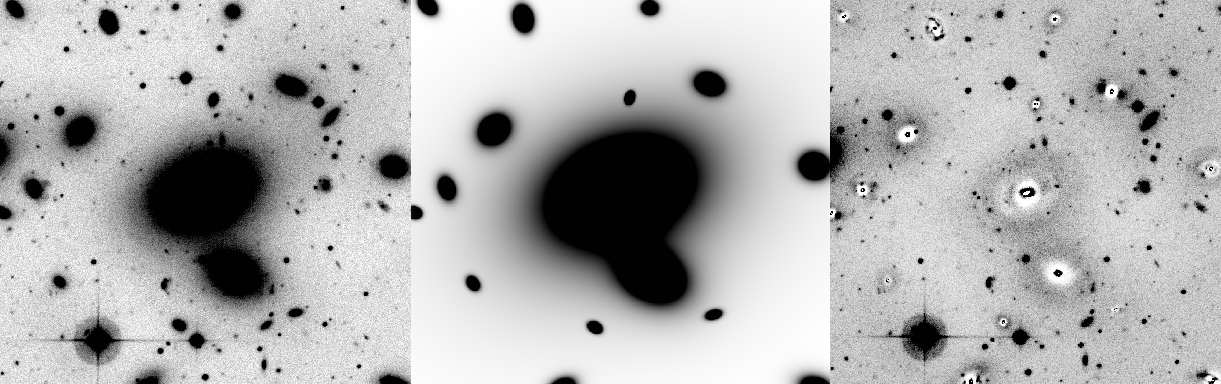
\includegraphics[width=15cm]{images/galfit.png}
\caption[Galfit results for Abell 754]{Galfit procedures for Abell 754. Left: Original image in ``zscale" with the BCG expanding across a significant region of the central area. Middle: The models fitted by \texttt{GALFIT} for all the selected cluster galaxies. Right: Residual image after the subtraction of the model galaxies. Note that the saturated star is not in the \texttt{GALFIT} models since it is simply masked out with the segmentation image.}
\end{figure}

These procedures are done over all the images and their 4 filters, which will allow us to make color images and discriminate between objects of the same color that could be lensing candidates as explained in the next section. For every cluster the images have the same spatial scale and are centered at the same exact location so we can use the same fitting models for every filter as seen in Figure [4.3]

\begin{figure}[H]
\centering
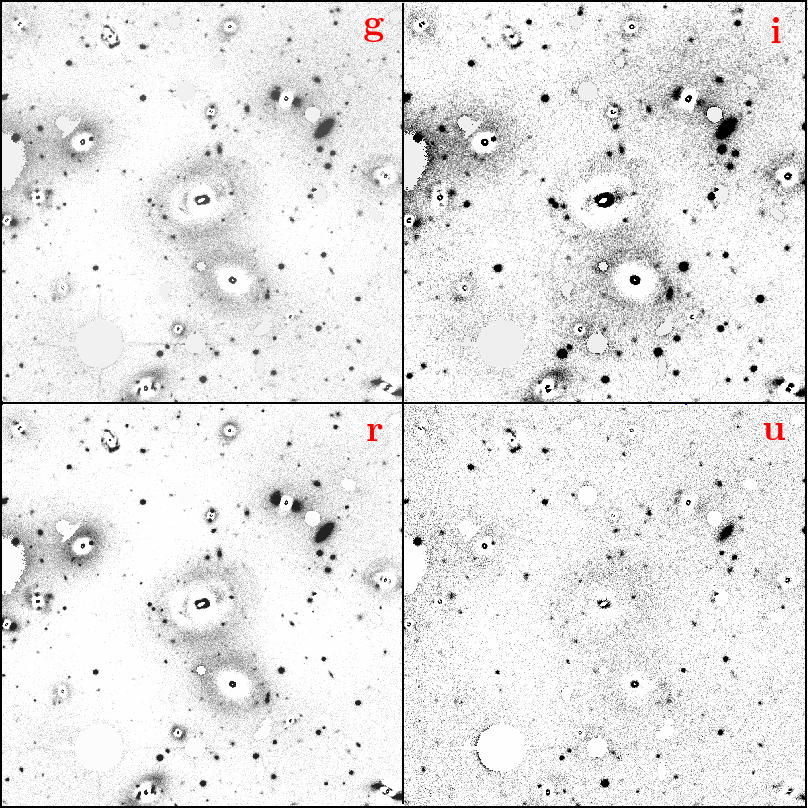
\includegraphics[width=12cm]{images/filters_A754.png}
\caption[All filters' results for Abell 754]{\texttt{GALFIT} results for the four availabe filters ($g,i,r,U$ respectively) of Abell 754 displayed in zscale. Note that depending on the filters some objects appear to be brighter or fainter and that will pay an important role in the creation of the color images and the photometric redshifts explained in the following sections.}
\end{figure}

The same procedure is applied on all the clusters. One of the most interesting targets of our sample is the cluster Abell 1413 (located at $z=0.143$) which has a prominent arc as seen in Figure [4.4] (although this cluster lacks of the $U$ band image). 

\begin{figure}[H]
\centering
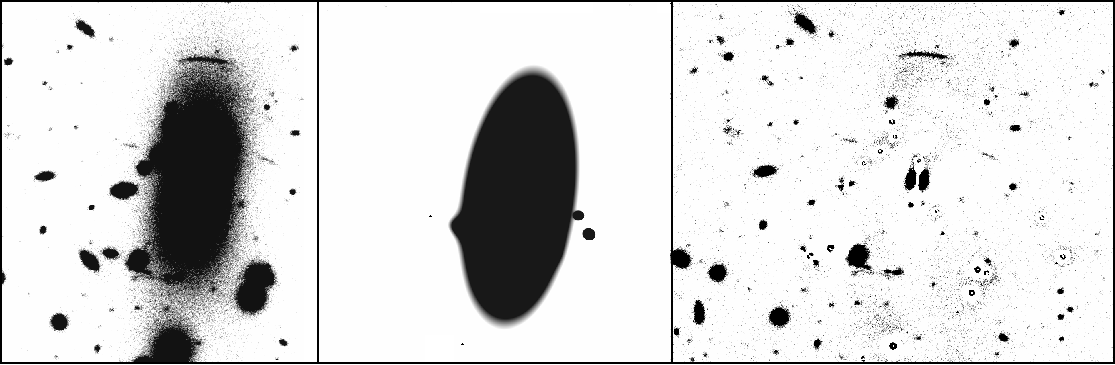
\includegraphics[width=15cm]{images/A1413.png}
\caption[Galfit results for Abell 1413]{Galfit procedures for  Abell 1413. Left: Original image in ``zscale" with the BCG. Middle: The models fitted by \texttt{GALFIT} for all the selected cluster galaxies. Right: Residual image after the subtraction of the model galaxies. This cluster in particular has many non-cluster memebers so fewer objects need to be subtracted.}
\end{figure}

\section{Color images} 

We use \texttt{IRAF} to make the color images using our $g,r,U,i$ bands. Let's keep using Abell 754 which is a low redshift galaxy ($z=0.054$) cluster with a calculated mass of $\text{M}_{200}=9.8\times 10^{15}$ $\text{M}_{\odot}$ (\textcolor{blue}{Sifon et al.} \citeyear{Reference9})

Here we take an isothermal sphere to model the Einstein ring for an assumed distance of background objects of $z=0.5$. We made a color image of the original center of the cluster without subtracting the BCG in order to differentiate between cluster members from background galaxies and field stars. This allows us to fit only the cluster galaxies. 

\begin{figure}[H]
\centering
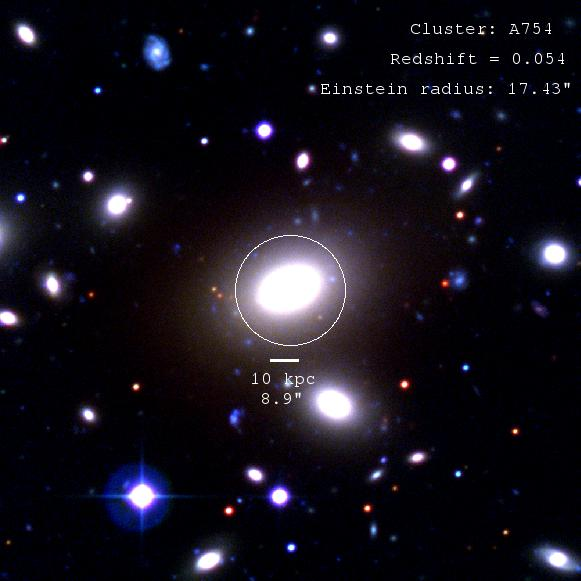
\includegraphics[width=12cm]{images/cA754.jpg}
\caption[Color image of A754]{Color image of A754 cluster (filters $i,g,U$) with its Einstein radius calculated for an isothermal sphere of a background object at $z=1$.}
\end{figure}

After choosing the galaxies that belong to the cluster by comparing their relative colors, we subtracted them using \texttt{GALFIT} and made the color image again changing the scaling values with the task \texttt{CONVERT} of \texttt{IRAF} so that we see can see the color contrast to search for good candidates of lensed objects. By looking at this reduced color image, we have another visual constraint to choose the clusters in which it would be worth to do photometric redshifts and search for objects with the same redshift in different locations around the very center of the BCG (object that has suffered strong lensing). 

\begin{figure}[H]
\centering
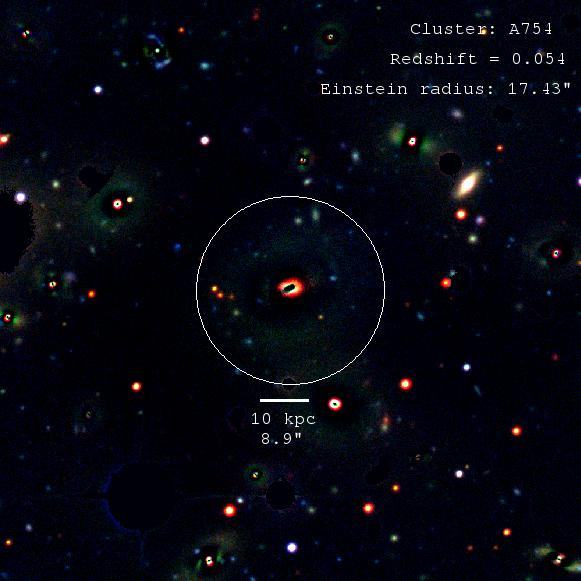
\includegraphics[width=12cm]{images/cA754_galfit.jpg}
\caption[Color image of A754 after fitting the bright objects]{Color image of A754 cluster (filters $i,g,U$) after the subtraction of the bright cluster galaxies.}
\end{figure}

The $i,r,g$ color image of the cluster Abell 1413: (this needs to be fixed)

\begin{figure}[H]
\centering
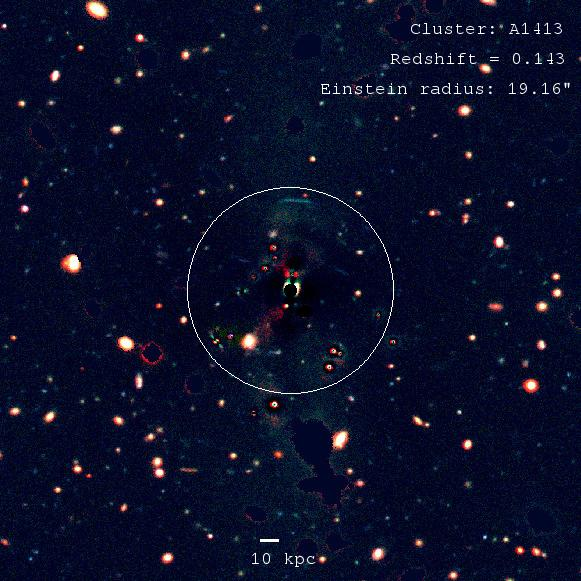
\includegraphics[width=15cm]{images/A1413_ring.jpg}
\caption[Einstein ring in color image of A1413]{Einstein ring in color image of Abell 1413.}
\end{figure}

Because we have 4 bands we were able to make different color images to see the contrast and make combinations that would allow us to see better the very red and very blue objects, hoping to find objects with the same colors that would be good candidates for lensed objects. Figure [4.8] displays the $g,r$, $i,r,g$ and $i,g,U$ color images for three clusters (Abell 961, Abell 2703 and Abell 1033). 

\begin{figure}[H]
\centering
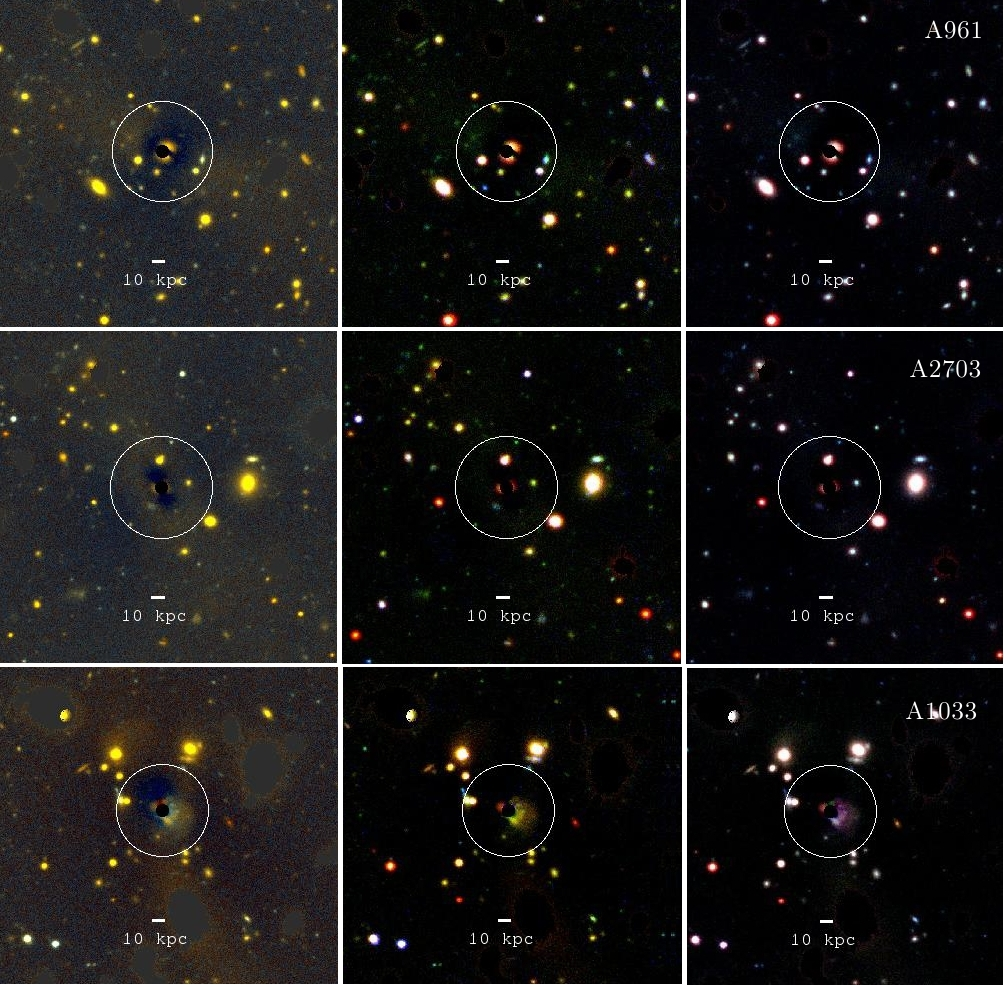
\includegraphics[width=15cm]{images/full_small.jpg}
\caption[Color images for various clusters]{Different color images for different combination of the $g,r,U,i$ filters for the clusters Abell 961, Abell 2703, Abell 1033. Left column for the images constructed only with the $g$ and $r$ filter, central column for $i,g,r$ and right column for $i,g,U$.}
\end{figure}

\section{Star-galaxy determination}

The first step in determining the photometric redshifts is to discriminate between field stars and the galaxies of the clusters so in order to do this, we used some of the parameters found by \texttt{SEXTRACTOR} that allow us to constraint the fitted data. These are \texttt{class-star}, \texttt{flux\_radius}, and \texttt{FWHM} (full width half maximum). Class-star uses the neural network star/galaxy of \texttt{SEXTRACTOR} that will give values close to 1 for stars and 0 for galaxies. \texttt{flux\_radius}, and \texttt{FWHM} are closely related to each other and give the radius which contains half of the light of the object so it will be small for stars and bigger for extended objects.

In order to extract the same objects and make the segmentation masks for the desired objects in the different filters, we used \texttt{SEXTRACTOR} on dual mode and made aperture photometry on each of the relevant objects. Figure [4.9] shows the color magnitude diagram for Abell 754 where we used a zero point magnitude of 30.

\begin{figure}[H]
\centering
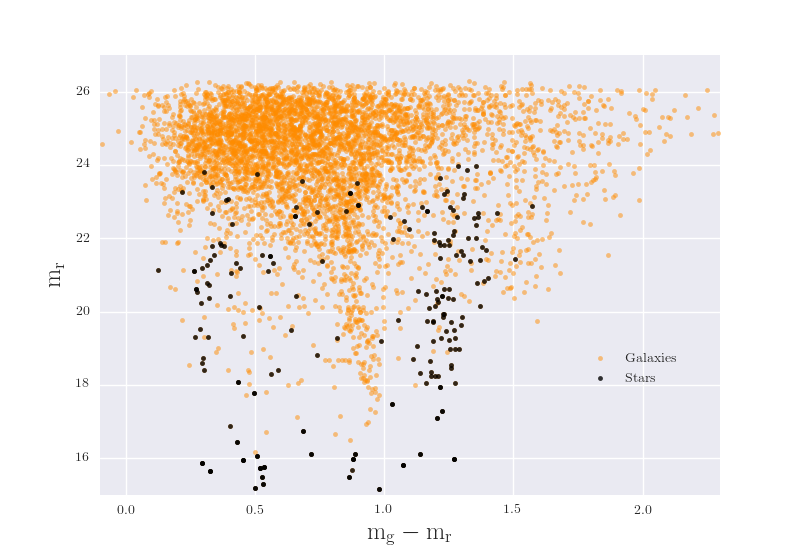
\includegraphics[width=12cm]{images/color_mag.png}
\caption[Color Magnitude diagram of Abell 754]{Color Magnitude diagram of Abell 754 with the differentiation of stars from galaxies.}
\end{figure}

We can also discriminate the stars from galaxies using the radius that contains most of the flux. Figure [4.10] shows the galaxies and stars in the mag vs \texttt{Flux\_rad} plane.

\begin{figure}[H]
\centering
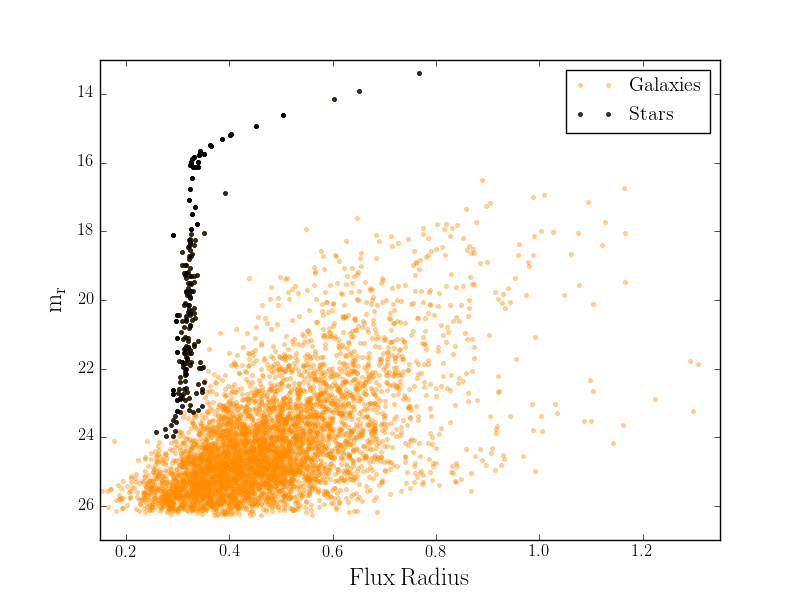
\includegraphics[width=12cm]{images/mag_vs_flux_rad.png}
\caption[Magnitude vs Flux radius of Abell 754]{Magnitude vs Flux radius of Abell 754 to identify the galaxies using the criteria of their flux distribution.}
\end{figure}

\section{Photometric Redshifts}

Using multi band photometry data to get redshifts (Photometric redshifts) is not only a useful method to get redshifts of fainter objects than accessible by spectroscopy, but also because the efficiency in terms of the number of objects with redshift estimates per unit telescope time is largely increased. Given the characteristics of our data (four bands with similar depth), getting photo-$z$'s of the background objects after the subtraction of the BCG's could in principle help us find lensed galaxies (background objects with the same redshift could be the same galaxy located at different locations so they are good lensing candidates).

In order to calculate the photometric redshifts we must make very accurate photometry on the four bands trying to minimize the errors associated to the removal of the light from the BCG that causes the photometry methods to overestimate or underestimate the background thus corrupting the output magnitudes. As seen in Figure [4.11], the background in the vicinity of some of the objects is over removed after the subtraction of the light of the BCG, so this effect would cause objects with the same real redshift (lensed background galaxies) to have different redshifts after running the photo-$z$ code.

\begin{figure}[H]
\centering
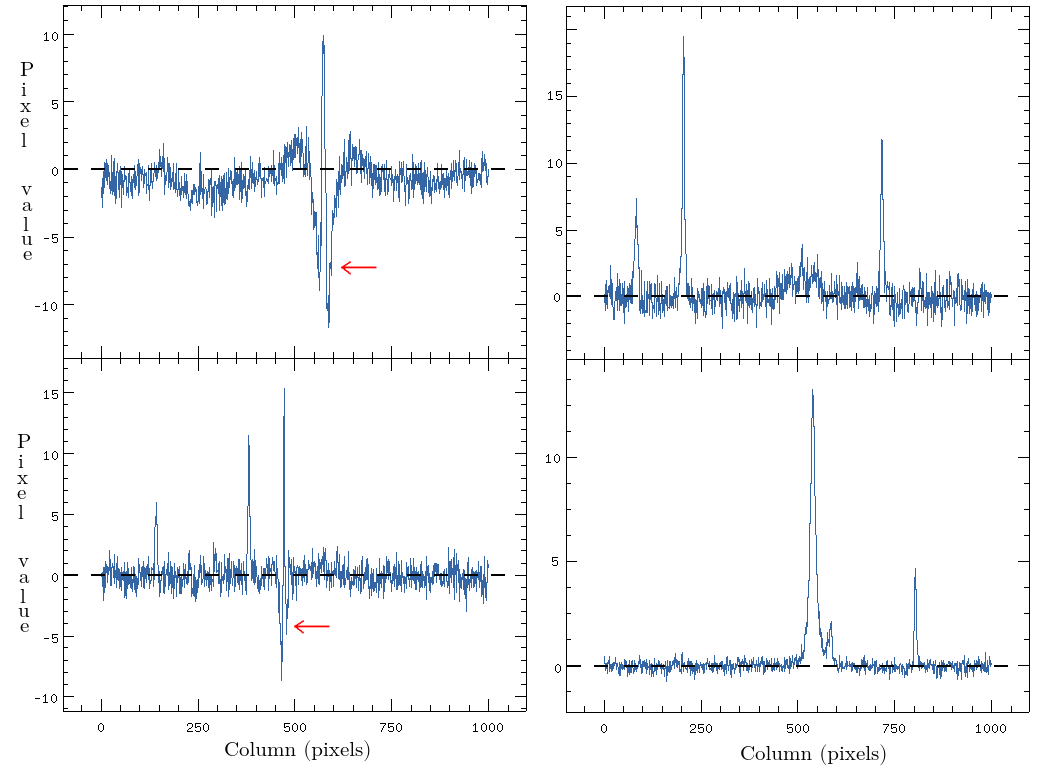
\includegraphics[width=15cm]{images/horizontal_cuts.png}
\caption[Horizontal cuts to show overestimated background on Abell 1068]{Horizontal cuts on cluster Abell 1068 for four random regions. On the left, objects with an overestimated background (indicated with the red arrows) where the values of the surroundings go well below zero. On the right, objects surrounded by a more accurate and smooth background.}
\end{figure}

In order to avoid this problem, we applied different methods for the photometry of the reduced data with a careful local background determination in every case. The very first approach (just for reference) was simply aperture photometry using \texttt{SEXTRACTOR} with the default parameters, the other methods were more precise and were made using the aperture photometry routines of \texttt{PHOTUTILS}. The first method is making aperture photometry with an annulus enclosing the surrounding background of every galaxy, the second method is choosing a fixed background (the mean value found with \texttt{IMSTATISTICS} of \texttt{IRAF}) and use it as the value for all the apertures, the third one is the average between the fixed background and the background value found in the annulus surrounding the objects. Figure [4.12] shows the objects on which we applied the photometry experiments for the galaxy cluster Abell 754.

\begin{figure}[H]
\centering
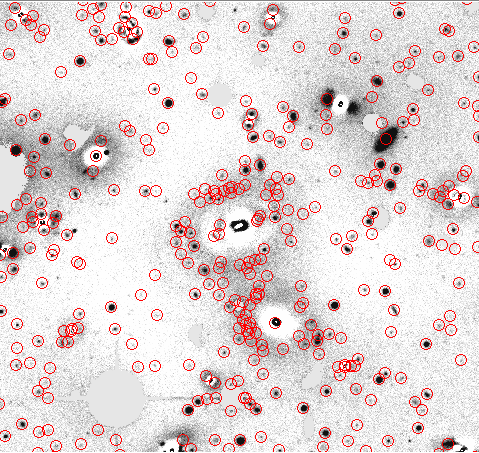
\includegraphics[width=15cm]{images/aperture_photometry.png}
\caption[Apertures for the aperture photometry procedures on Abell 754]{Apertures for the aperture photometry procedures for the core of galaxy cluster Abell 754. This is the full sample of objects without the discrimination of stars and galaxies from the cluster.}
\end{figure}

The physical coordinates of the objects  were obtained with \texttt{SEXTRACTOR} since the filtering and identification of the objects is quite straight forward. Once we have obtained the magnitudes of the galaxies in our four filters, and have chosen the method that yields the most satisfactory results (in our case the average between the fixed background and the one associated to the annuli), we can measure the photometric redshift of the galaxies in the inner region of the cluster.

We use the photometric redshift code \texttt{EAZY}  by \textcolor{blue}{Brammer et al.} (\citeyear{Reference22}) which uses an extensive collection of spectral energy distributions for galaxies in the range $0<z<4$. It basically finds discontinuities such as Lyman break ($1200$ \AA) and the Balmer break ($4000$ \AA) in the SED of galaxies which give a constraint on the redshift. Fortunately, the code includes library from CFHT in the $i$ and $U$ bands but doesn't have the filters in the $g$ and $r$ bands so we used the SUBARU survey filter information to be able to compute the photometric redshifts using the four bands. The use of a $r$ band magnitude prior allows the code to correctly calibrate the redshifts since the location of the break might be misunderstood by the code. Figure [4.13] shows our obtained photometric redshifts for the cluster Abell 754 (376 galaxies after filtering out field stars and removing the brightest galaxies that belong to the cluster) for all of our photometry experiments and compared them to the ones found by Remco Van der Burg (private communication) on a larger field for the same cluster. 

\begin{figure}[H]
\centering
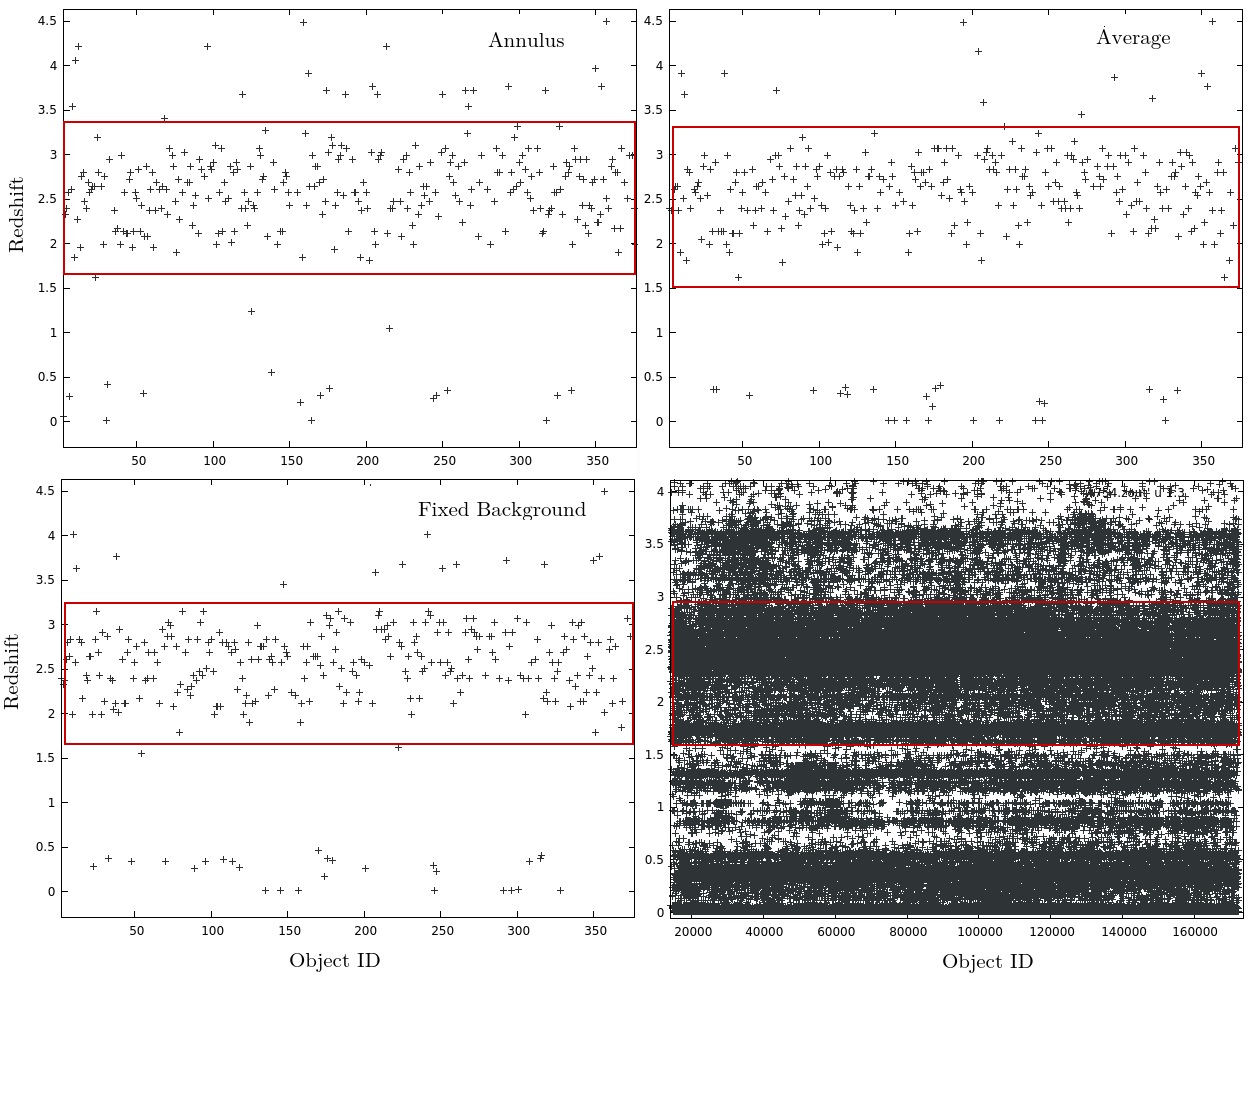
\includegraphics[width=15cm]{images/photo_z_red_squares.png}
\caption[Photometric redshift results for Abell 754]{Photometric redshift results for Abell 754. Top left: Results for the photometry method in which the background was determined with an annulus around the objecrs. Bottom right: Using a fixed background (mean of the background). Top left: An average between the two other methods. Bottom left: Van der Burg's results for the photo-$z$'s for a much larger sample (188,964 objects). The red squares represent the regions of the ``junk" data which we can neglect for the lensing analysis. The green squares indicate the regime of the background galaxies where we want to look for lensing candidates.}
\end{figure}

One last filter has to be applied to the data. Since the calculated redshifts should be consistent with the expected values according to the COSMOS experiment, we need to select only the galaxies that have low redshifts (they are more suitable for being lensing candidates in the sample). For this, we only select the galaxies whose photo-$z$'s are in the low regime as shown with the green squares in Figure [4.13] and use their respective ID to identify their corresponding magnitude. 

Now that we have selected the magnitude in every filter for the filtered galaxies, we analyze their flux distribution by ploting their arbitrary flux against $\lambda$, taking as reference the effective wavelengths of the filters $U,g,r,i,$ and see the shape of their distribution. If we find objects with very similar flux distributions (similar behavior in the plot), then we might check their coordinates and see weather this difference is a coincidence or they can be in fact the same object.

Figure [4.14] shows the magnitude distribution for the final filtered sample of galaxies surrounding the BCG of Abell 2064. We see that two objects present a very similar magnitude distribution so it is an interesting target to look at. 

\begin{figure}[H]
\centering
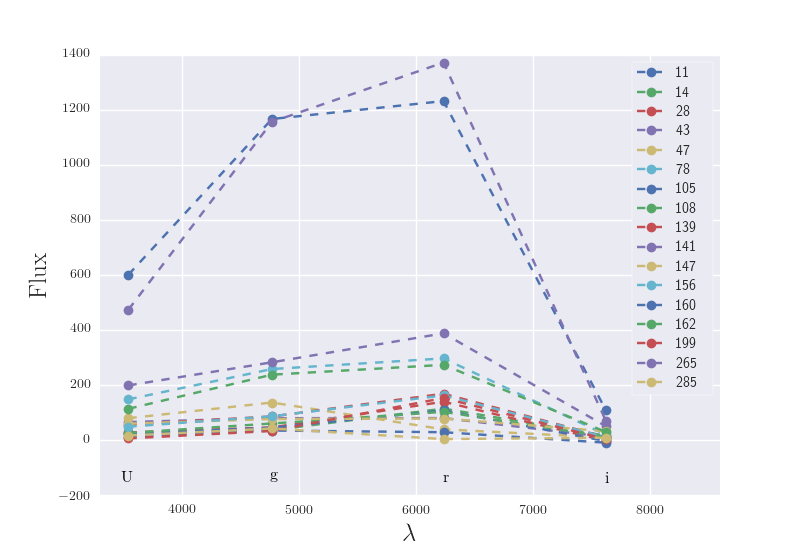
\includegraphics[width=15cm]{images/magnitude_distribution_A2064.png}
\caption[Magnitude distribution of galaxies in Abell 2064]{Magnitude distribution for galaxies with low photometric redshift and their respective ID for cluster Abell 2064. Note that the only 17 galaxies belong to the low redshift regime out of the 320 galaxies over which we ran the photo-$z$ code.}
\end{figure}

Even though the two most prominent plots in Figure [4.14] appear to have a bad flux distribution, they are still interesting candidates since we care about the similarities between their distributions instead of how well behaved they are. Figure [4.15] shows the location of the objects that have a similar flux distribution with their corresponding ID in two different color images ($i,g,u$ and $i,r,g$).

\begin{figure}[H]
\centering
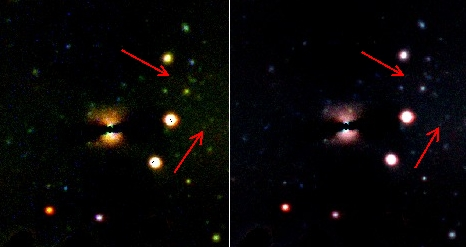
\includegraphics[width=15cm]{images/candidates.jpg}
\caption[Lensing candidates Abell 2064]{Lensing candidates in Abell 2064. Left: Color image made with the $i,g,u$ filters. Right: Color image made with the $i,r,g$ filters. Note that an inspection by eye would miss the objects because they are very faint.}
\end{figure}

In principle, both galaxies seem to have a very related flux distribution so the two points seem to be good candidates for a more precise analysis, but unfortunately the photometric redshift for both galaxies is not similar and they are very faint to give trustworthy results, specially with the $U$-band data so it is discarded as a good candidate. % Data and analysis

\lhead{\emph{Conclusions}} 
\chapter{Conclusions}

The COSMOS experiment shows that we should expect a few lensed objects in the spatial scale and with the sensitivity of our data. Even though the number is small, a proper subtraction of the BCG would allow us to see a few objects in the innermost region of the clusters. In our sample we indeed find a few background galaxies (using the photo-$z$'s) but none of them are suitable lensing candidates.

Perhaps the most important conclusion in this work is that for the purpose of characterizing IMFs in massive systems, it is better to use galaxies than BCGs because the stellar contribution is less important in the latter, even in the small radial distances from the centre. The overwhelming dominance of DM in the centre of galaxy clusters makes the determination of the stellar content harder since we can't assume that mass follows light thus lensing doesn't provide direct information about the baryonic mass. In the case of galaxies, even though the spatial scales in which stellar content is important are very small, they allow for a better constraint using gravitational lensing since these distances are close to the Einstein rings.

The most clear strong lensing feauture in our sample is in the cluster Abell 1413 where a long arc is clearly seen. It is a good candidate for follow up studies. Unfortunately, in our sample we don't have $U$ band data for this cluster so the characterization of the lens couldn't be done properly. 

Another interesing result in our observational procedures is that the subtraction of the BCGs shows that (at least in our sample) the inner region doesn't have a general trend, some objects are very crowded, some are not.

photometry in the cluster after the subtraction of the BCG is complicated so it has to be really well done otherwise the photozs are going to be shit

our spatial scale where the stellar contribution is still important is in the very center, so the Einstein rings that are in that region are the ones for low redshift objects so those are the objects we expect in experiments like this one.

\section{Possible improvements}

follow up studies like (reference Smiths papers) need to have spectroscopy to compare the photometric redshifts.

more filters to have better photo-$z$

take into account the central mass in this system which also affects the photometry of them

first identify a clear candidate and then do the follow up studies about the IMF

\newpage
\lhead{\emph{Appendix}} 
\begin{appendices}
\textbf{{\LARGE Appendix}}

$\qquad$

\textbf{Isothermal Sphere} 

Summary of isothermal sphere:

\begin{equation}
\rho(r)=\frac{\sigma^2}{2\pi Gr^2}
\end{equation}

\begin{equation}
\Sigma(\xi)=\frac{\sigma^2}{2G\xi}
\end{equation}

The Einstein radius:

\begin{equation}
\xi_{E}=4\pi\left(\frac{\sigma}{c}\right)^{2}\frac{D_{ds}}{D_{s}}
\end{equation} 
 
\textbf{NFW profile formalism}
 
The NFW density profile is 

\begin{equation}
\rho(r)=\frac{\delta_{c}\rho_{c}}{(r/r_{s})(1+r/r_{s})^{2}}
\end{equation}

where the characteristic over density (dimensionless quantity) is given by:

\begin{equation}
\delta_{c}=\frac{200}{3}\frac{c^{3}}{\ln{(1+c)}-c/(1+c)}
\end{equation}

The mass of an NFW halo contained within a radius of $r_{200}$ is:

\begin{equation}
\text{M}_{200}=\text{M}(r_{200})=\frac{800\pi}{3}\rho_{c}r^{3}_{200}=\frac{800\pi}{3}\frac{\bar{\rho}(z)}{\Omega(z)}r^{3}_{200}
\end{equation}

The concentration parameter $c$ is strongly correlated with Hubble type, $c=2.6$ separating early from late-type galaxies. Those galaxies with concentration indices $c>2.6$ are early-type galaxies reflecting the fact that the light is more concentrated towards their centres, its formal definition in terms of the virial and characteristic radius is $c=r_{200}/r_{s}$.

\textcolor{blue}{Dutton \& Maccio} (\citeyear{Reference23}) (in continuation of previous studies such as \textcolor{blue}{Mu\~noz Cuartas et al.} \citeyear{Reference12}), made simulations of halo masses from dwarf galaxies to galaxy clusters and find constraints on the concentration parameter for different redshifts, the relation between the concentration parameter with redshift and virial mass is shown in Figure [1].

\begin{figure}[H]
\centering
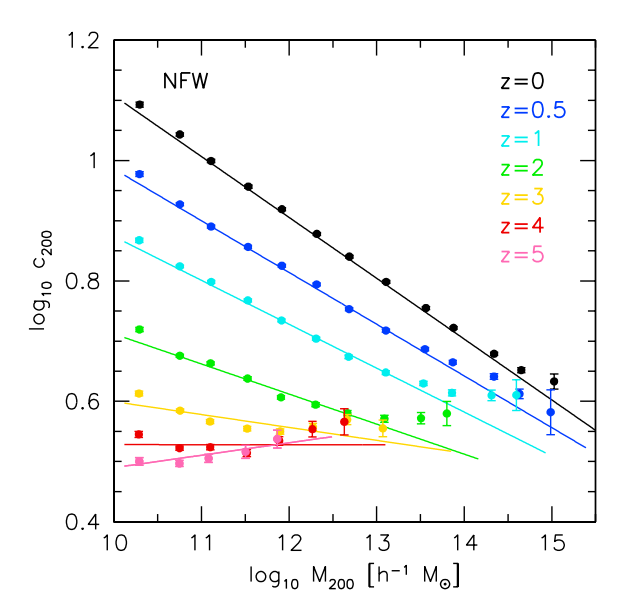
\includegraphics[width=10cm]{images/dutton.png}
\caption[Evolution of the concentration mass relation]{Evolution of the concentration mass relation, by \textcolor{blue}{Dutton \& Maccio} (\citeyear{Reference23}).}
\end{figure}

The surface mass density in the NFW profile (\textcolor{blue}{Wright \& Brainerd}, \citeyear{Reference4}) is given by:

\begin{equation}
\Sigma_{\text{NFW}}(x) = \left\lbrace
\begin{array}{lll}
\frac{2r_{s}\delta_{c}\rho_{c}}{\left(x^{2}-1\right)}\left[1-\frac{2}{\sqrt{1-x^{2}}}\arctanh\sqrt{\frac{1-x}{1+x}}\right] & (x<1)\\\\
\frac{2r_{s}\delta_{c}\rho_{c}}{3} & (x=1)\\\\
\frac{2r_{s}\delta_{c}\rho_{c}}{\left(x^{2}-1\right)}\left[1-\frac{2}{\sqrt{x^{2}-1}}\arctan\sqrt{\frac{x-1}{1+x}}\right] & (x>1)
\end{array}
\right.
\end{equation} 

so from the critical density:

\begin{equation}
\rho_{c}=\frac{3H^2(z)}{8\pi G}
\end{equation}

$H(z)=H_{0}(1+\Omega z)^{3/2}$

But we are more interested in the enclosed mass which can be done by integrating the surface mass density:

\begin{equation}
\text{M}(R)=\int_{0}^{R}2\pi R\Sigma(R)dR
\end{equation}

The radial dependence on the shear is:

\begin{equation}
\gamma_{\text{NFW}}(x) = \left\lbrace
\begin{array}{lll}
\frac{r_{s}\delta_{c}\rho_{c}}{\Sigma_c}g_{<}(x) & (x<1)\\\\
\frac{r_{s}\delta_{c}\rho_{c}}{\Sigma_c}\left[\frac{10}{3}+4 \ln \left(\frac{1}{2}\right)\right] & (x=1)\\\\
\frac{r_{s}\delta_{c}\rho_{c}}{\Sigma_c}g_{>}(x) & (x>1)
\end{array}
\right.
\end{equation} 

where: 

\begin{equation}
g_{<}(x)=\frac{8 \arctanh \sqrt{\frac{1-x}{1+x}}}{x^{2}\sqrt{1-x^{2}}}+\frac{4}{x^{2}} \ln \left(\frac{x}{2}\right)-\frac{2}{\left(x^{2}-1\right)}+\frac{4 \arctanh \sqrt{\frac{1-x}{1+x}}}{\left(x^{2}-1\right)\left(1-x^{2}\right)^{1/2}}
\end{equation}

\begin{equation}
g_{<}(x)=\frac{8 \arctan \sqrt{\frac{x-1}{1+x}}}{x^{2}\sqrt{x^{2}-1}}+\frac{4}{x^{2}}\ln \left(\frac{x}{2}\right)-\frac{2}{\left(x^{2}-1\right)}+\frac{4 \arctan \sqrt{\frac{x-1}{1+x}}}{\left(x^{2}-1\right){}^{3/2}}
\end{equation}  

For reference, Figure [2] shows strong systematic variation of the IMF in early-type galaxies as a function of their stellar mass-to-light ratio, producing differences up to a factor of three in mass by \textcolor{blue}{Cappellari et al.} (\citeyear{Reference19})

\begin{figure}[H]
\centering
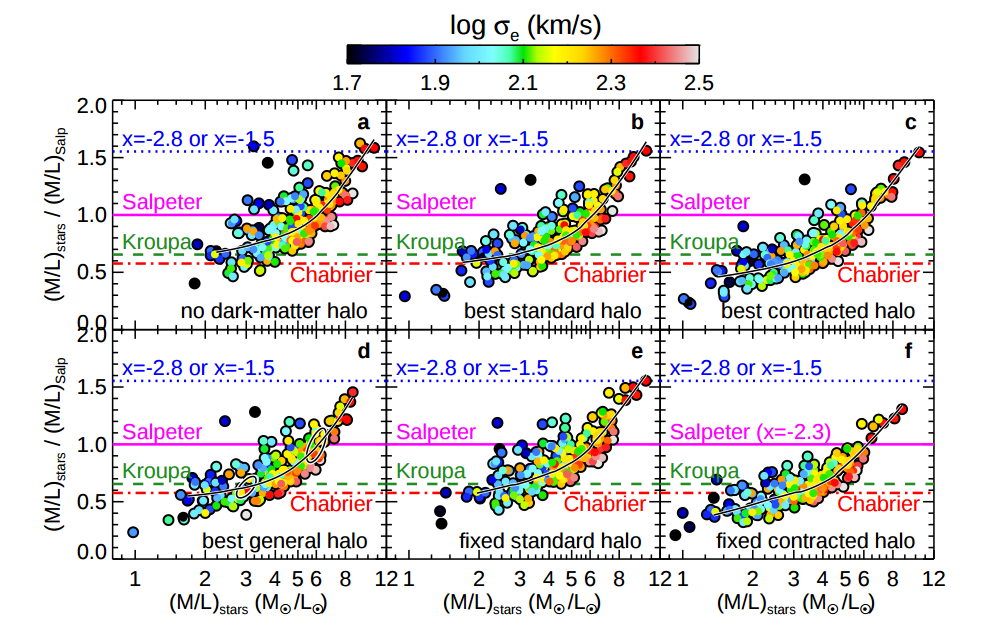
\includegraphics[width=12cm]{images/IMFs_paper.png}
\caption[The systematic variation of the IMF in early-type galaxies.]{The systematic variation of the IMF in early-type galaxies, \textcolor{blue}{Cappellari et al.} (\citeyear{Reference19}).}
\end{figure}
 
\end{appendices} % Conclusions

\label{Bibliography}
\lhead{\emph{Bibliography}}  % Change the left side page header to "Bibliography"
\bibliographystyle{unsrtnat}  % Use the "unsrtnat" BibTeX style for formatting the Bibliography
\bibliography{Bibliography}  % The references (bibliography) information are stored in the file named "Bibliography.bib"

\end{document} 
